% ------------------------------------------------------------- 
% Arquivo :  relatório modelo                                        
% ------------------------------------------------------------- 
% O percentual(%) serve para incluir comentários: 
% tudo o que fica à direita dele não é interpretado pelo LaTex
% Linhas e espaços em branco também **NÃO** são
% interpretadas pelo LaTex

%% As intruções seguintes são o cabeçalho e devem estar antes do
%% \begin{document}

%\documenclass: mandatorio, indica o tipo/formato de documento
\documentclass[brazilian,12pt,a4paper,final]{article}
% tamanhos de fontes: 10pt, 11pt ou 12pt
% opções de estilo (padrões): article, report, book, slide, letter (artigo, relatorio, livro, apresentação de slides, carta)




%% Pacotes extras (opcionais):

% *babel* contem as regras de ifenização
\usepackage[brazil]{babel}

% *t1enc* permite o reconhecimento dos acentos inseridos com o teclado
%\usepackage{t1enc}

% *inputenc* com opção *utf8* permite reconhecimento dos caracteres com codificação UTF8, que é padrão dos esditores de texto no Linux. Isso permite reconhecimento automático de acentuação.
\usepackage[utf8]{inputenc}


% *graphicx* é para incluir figuras em formato eps 
\usepackage{graphicx} % para produzir PDF diretamente reescrever esta linha assim: \usepackage[pdftex]{graphicx}

% *color* fontes soloridas
\usepackage{color}
%%% fim do cabecalho %%%

\pagestyle{empty}
\title{Métodos Computacionais da Física A - prova}
\author{Aluno: Átila Leites Romero - Matrícula: 144679 \\ IF-UFRGS}

\begin{document}
\maketitle

\section{} 
\begin{verbatim}
cd /home/metcompA_2010-2_Carolina/atilaromero/
mkdir prova1
cd prova1/
emacs -nw arqprova1.tex
\end{verbatim}

\section{} 
\begin{verbatim}
max=x[1]
med=0
i=1
enquanto i<=1000:
  med+=x[i]
  if x[i]>max:
    max=x[i]
  i++
med=med/1000
imprima max
imprima med
\end{verbatim}

\section{} 
\begin{verbatim}
i=0 j=7 k=0 
i=3 j=10 k=6 
i=6 j=16 k=12 
i=9 j=25 k=18 
i=12 j=37 k=24 
\end{verbatim}

\section{} 
Variando $N$ de 1 a 200 e $x = 0.95$, os dados obtidos foram:
\begin{figure}[htbp]
\begin{center}
\rotatebox{-90}{\resizebox{8.0cm}{!}{\includegraphics{0.95.dat.eps}}}
\caption{f(0.95) vs N}
\label{fig_rotacao}
\end{center}
\end{figure}

Nota-se que, conforme $N$ aumenta, os valores de $f(x)$ aproximam-se do resultado correto. 
Por isso, para valores muito próximos de 1 são necessários valores muito altos de $N$ para que seja encontrado o resultado.
Enquanto para $x = 0.2$ o resultado é encontrado em aproximadamente em $N = 10$, quando $x = 0.95$ o resultado está longe de ser alcançado em $N = 100$.
O segundo gráfico mostra esta diferença.

\begin{figure}[htbp]
\begin{center}
\rotatebox{-90}{\resizebox{8.0cm}{!}{\includegraphics{0.2.dat.eps}}}
\caption{f(0.2) vs N}
\label{fig_rotacao}
\end{center}
\end{figure}



\begin{verbatim}
\end{verbatim}

\end{document}

